\section{\mc 目的}
\subsection{\mc モチベーション}
BCIを構築する基本的なアプローチは以下の二種に大別できる。
\begin{itemize}
    \item 神経科学的アプローチ:EEGに生じる特定の現象を特徴量として用い、分類器を構築する。
    \item 機械学習的アプローチ:特徴量抽出自体を統計的な処理によって行い、分類器を構築する。
\end{itemize}
神経科学的アプローチでは運動想起時のERDや運動前に生ずる運動準備電位、
点滅刺激を視認した際のSteady State Visual Evoked Potential(SSVEP)など、
脳神経科学において既知の現象を精度よく検出することでBCIの構築を目指す。
これらの神経科学的アプローチは、EEGから人間の脳活動状態をある分類可能であるかを調べる上で
非常に重要な役割を担うと考えているが、
BCIを実際に応用する場面を考慮すると
個々人のEEGの解析と適切な特徴量の選定、更に分類器の設計も別途必要となり
今後の応用範囲の拡大を考える上では限界がある。
また、仮にタスク間でのEEGの違いを可視化したい場合や、
脳機能自体を解明したい場合には綿密なEEGの解析は有効であるが、
その際には解析はあくまで人間が解釈する手段であり、
解析のために処理された信号がそのままBCIを用いる際の特徴量として有望だとは限らない。
なぜなら人間がデータを解釈、あるいは可視化できるような形に加工することで
分類に有用な情報が失われている可能性もあるためである。

一方で機械学習的なアプローチでは、綿密なEEGの解析を実施するか否かに関わらず、
例えば左手を動作させる場合と右手を動作させる場合とでは脳の活動は事実異なっているため、
その違いを顕著に示す信号の表現の獲得を機械学習や統計的信号処理によって行い、
その後、更に分類器を機械学習によって設計することでBCIを構築する。
しかし、統計的信号処理や機械学習に基づく
特徴量抽出手法と分類手法にも数多くの種類が存在するため、
実際にBCIを構築する際には複数の手法とその組み合わせに関しての検討に
多くの時間を要することとなる。
BCIの一部として用いられる信号処理、あるいは機械学習手法の代表を以下に記す。
この中の幾つかは第\ref{chapter:BCIのための要素技術}章にて解説する。
\begin{itemize}
    \item Laplacian Filter(LF)
    \item Principal Component Analysis(PCA)
    \item Independent Component Analysis(ICA)
    \item Canonical Correspondence Analysis(CCA)
    \item Common Spartial Pattern(CSP)
    \item バンドパスフィルタバンク
    \item フーリエ変換
    \item ウェーブレット変換
    \item 自己回帰モデル
    \item Emperical Mode Decomposition(EMD)
    \item Linear Discriminat Analysis(LDA)
    \item Support Vector Machine(SVM)
    \item Logistic Regression(LR)
\end{itemize}

\subsection{\mc 目的と貢献}
神経科学的アプローチのように個人事に綿密なEEGの解析を行う必要性が残る限り、
専門家が常にいる医療の現場などの特定の分野でのみしかBCIの発展は望めない。
また現在の機械学習的アプローチでBCIを構成する場合には、
考えうる手法の組み合わせは無数にあるため、決定的なアーキテクチャが存在しないと言える。
そこで、本研究の目的として
神経科学的アプローチと機械学習的アプローチの両方の問題点を同時に解決するために、
個人事のEEGの解析を行うこと無く入力から出力までのBCIの構成を
データから一貫して推定する``End to End学習''を提案し、BCIを構築する。

End to End学習を達成するために、
音声認識と画像認識の分野で既に大きな成功を収めている
ニューラルネットワークに着目した。
BCIとして考えうる構成と、ニューラルネットワークを用いたBCIの構成図を図\ref{fig:BCIpattern}に示す。
\begin{figure}
    \centering
    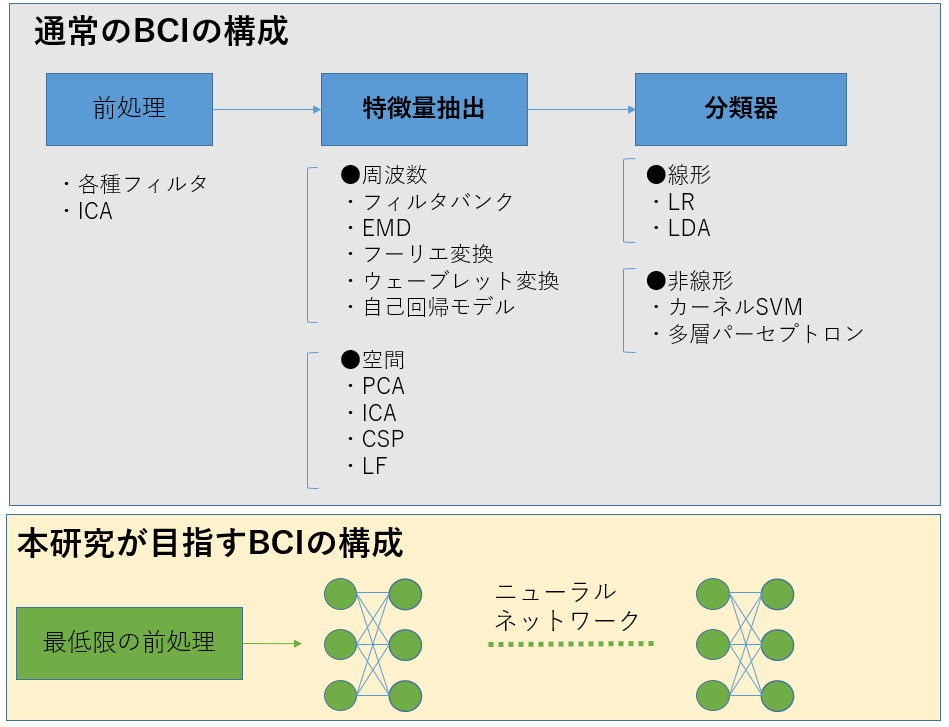
\includegraphics[width=12cm]{images/BCIpattern.PNG}
    \caption{従来のBCIの構成と本研究が目指すBCIの構成}
    \label{fig:BCIpattern}
\end{figure}
またEnd to End学習を提案することによって以下の項目について達成することを目標とした。
\begin{itemize}
    % \item タスク毎のEEGの解析の必要性を排除
    \item 各個人におけるEEGの解析の必要性を排除
    \item 人類に共通した一般的なBCIの可能性を示す
\end{itemize}
更に、今後のBCIの発展の準備として多数の被験者のEEGを用いてEnd to End学習したBCIが、
新規の被験者に対して適用可能かを検討し、適用可能となるような手法として転移学習\cite{転移学習}を提案する。

本研究によって人類に共通した一般的BCIの構築を行い、
新たな被験者に対して比較的少数のデータで、
一般的BCIから個人用BCIへキャリブレーションするBCIの構築の可能性が示唆される。

% ``各個人におけるEEGの解析の必要性を排除''はEnd to End学習の直接的な貢献であるが、
% 更に``人類に共通した一般的なBCIの可能性を示す''ことで基本的なBCIの大枠を獲得しておき、
% 個々人に応じて比較的少量のデータからキャリブレーションを行う
% 転移学習の可能性を示唆することができる\cite{転移学習}。


% また、ニューラルネットワークの応用研究が盛んな画像認識の分野では、
% 既に模範的なニューラルネットワークの構造が発見されており、
% 大量の画像によって事前学習を行い、
% 達成したい認識対象を絞り込んだ後に転移学習することで
% 手軽に高い性能の分類器が得られる。
% 従って、BCIにおいて模範的なニューラルネットワークの構築により
% 以下の事項が達成できる可能性が示唆される。
% 従って研究の成果によって以下の項目において貢献することができる。

% また、マルチモーダルなBCIの一部としても応用可能である。

% 更に、モデルの構築も含めハイパーパラメータの存在によって
% 試行錯誤の必要性も非常に高い。
% しかし、特徴量抽出手法や分類器自体を変更しながら様々な組み合わせを検討することに比べ、
% ニューラルネットワークの調整は単純作業である。
% また今後ハイパーパラメータの調整自体を自動化する、
% あるいは学習に組み込む方法も出現する可能性がある。


